%%%%%%%%%%%%%%%%%%%%%%% file template.tex %%%%%%%%%%%%%%%%%%%%%%%%%
%
% This is a general template file for the LaTeX package SVJour3
% for Springer journals.          Springer Heidelberg 2010/09/16
%
% Copy it to a new file with a new name and use it as the basis
% for your article. Delete % signs as needed.
%
% This template includes a few options for different layouts and
% content for various journals. Please consult a previous issue of
% your journal as needed.
%
%%%%%%%%%%%%%%%%%%%%%%%%%%%%%%%%%%%%%%%%%%%%%%%%%%%%%%%%%%%%%%%%%%%
%
% First comes an example EPS file -- just ignore it and
% proceed on the \documentclass line
% your LaTeX will extract the file if required
\begin{filecontents*}{example.eps}
%!PS-Adobe-3.0 EPSF-3.0
%%BoundingBox: 19 19 221 221
%%CreationDate: Mon Sep 29 1997
%%Creator: programmed by hand (JK)
%%EndComments
gsave
newpath
  20 20 moveto
  20 220 lineto
  220 220 lineto
  220 20 lineto
closepath
2 setlinewidth
gsave
  .4 setgray fill
grestore
stroke
grestore
\end{filecontents*}
%
\RequirePackage{fix-cm}
%
%\documentclass{svjour3}                     % onecolumn (standard format)
%\documentclass[smallcondensed]{svjour3}     % onecolumn (ditto)
\documentclass[smallextended]{svjour3}       % onecolumn (second format)
%\documentclass[twocolumn]{svjour3}          % twocolumn
%
\smartqed  % flush right qed marks, e.g. at end of proof
%
% \usepackage{mathptmx}      % use Times fonts if available on your TeX system
%
% insert here the call for the packages your document requires
\usepackage{latexsym}
\usepackage{graphicx}
\usepackage{amsmath, amssymb, amsfonts, mathtools}
\usepackage{enumerate}
\usepackage{algorithm, algpseudocode}
\usepackage{txfonts, pxfonts}
\usepackage{grffile}
\usepackage{caption, subcaption}
\usepackage{listings}
\usepackage[table, xcdraw]{xcolor}
\usepackage{rotating}
\usepackage{multirow}
\usepackage{chronology}
\usetikzlibrary{arrows, shapes}
\usepackage{tabularx}
\usepackage{hyperref}
\usepackage{libertine}
\usepackage{pgfgantt}
\usepackage{lscape}
\usepackage{enumitem}
\input amssym.def
\input amssym.tex
%
% please place your own definitions here and don't use \def but
\newcommand{\mmlcpt}{$mbMML_{CPT}$ }
\newcommand{\mbptmml}{$MBPT_{mml}$ }
\DeclareMathOperator*{\argmin}{arg\,min}
\DeclarePairedDelimiter\floor{\lfloor}{\rfloor}
\newcommand{\ci}{\mathrel{\text{\scalebox{1.07}{$\perp\mkern-10mu\perp$}}}}
\newcommand{\independent}{\perp\mkern-9.5mu\perp}
\newcommand{\notindependent}{\centernot{\independent}}
\newcommand{\qedwhite}{\hfill \ensuremath{\Box}}
\algnewcommand\algorithmicforeach{\textbf{for each}}
\algdef{S}[FOR]{ForEach}[1]{\algorithmicforeach\ #1\ \algorithmicdo}

\makeatletter
% Taken from http://ctan.org/pkg/centernot
\newcommand*{\centernot}{%
  \mathpalette\@centernot
}
\def\@centernot#1#2{%
  \mathrel{%
    \rlap{%
      \settowidth\dimen@{$\m@th#1{#2}$}%
      \kern.5\dimen@
      \settowidth\dimen@{$\m@th#1=$}%
      \kern-.5\dimen@
      $\m@th#1\not$%
    }%
    {#2}%
  }%
}
\makeatother

%
% Insert the name of "your journal" with
% \journalname{myjournal}
%
% This file can be modified and used in other conferences as long
% as credit to the authors and supporting agencies is retained, this notice
% is not changed, and further modification or reuse is not restricted.

\begin{document}

\title{Weak recursively simplicial graphs
%On checking Markov blankets consistency with DAGs via graph immoralization%\thanks{Grants or other notes
%about the article that should go on the front page should be
%placed here. General acknowledgments should be placed at the end of the article.}
}
%\subtitle{Do you have a subtitle?\\ If so, write it here}

%\titlerunning{Short form of title}        % if too long for running head

\author{First Author         \and
        Second Author \and
        Third Author
}

%\authorrunning{Short form of author list} % if too long for running head

\institute{F. Author \at
              first address \\
              Tel.: +123-45-678910\\
              Fax: +123-45-678910\\
              \email{fauthor@example.com}           %  \\
%             \emph{Present address:} of F. Author  %  if needed
           \and
           S. Author \at
              second address
}

\date{Received: date / Accepted: date}
% The correct dates will be entered by the editor

\maketitle

\section{Preliminary}

\begin{definition}
\label{def:subgraph}
Let $F=(V,E)$ and $F'=(V',E')$ be two graphs. If $V' \subseteq V$ and $E' \subseteq E$, then $F'$ is a \textbf{subgraph} of $F$ (and $F$ is a \textbf{supergraph} of $F'$), written as $F' \subseteq F$. If $F' \subseteq F$ and $F'$ contains all the edges $xy \in E$ with $x, y \in V'$, then $F'$ is an \textbf{induced subgraph} of $F$, written as $F' = F[V']$. 
\end{definition}

\begin{definition}
A \textbf{clique} is a subset of nodes in an undirected graph where every two distinct nodes are adjacent. 
\end{definition}

\begin{definition}
A \textbf{simplicial node} in an undirected graph is a node whose neighbours form a clique. 
\end{definition}

\begin{definition}
A graph $F=(V,E)$ is \textbf{recursively simplicial} if it contains a simplicial node $v_i$ and the induced subgraph $F[V\setminus \{v_{i}\}]$ is recursively simplicial. 
\end{definition}

\begin{definition}
A \textbf{simplicial node ordering} of a recursively simplicial graph $F=(V,E)$ is a sequence of nodes $\{v_1, \dots, v_n\}$, where $v_i$ is a simplicial node in the induced subgraph $F[V\setminus \{v_1,\dots, v_{i-1}\}]$.
\end{definition}

\begin{definition}
An \textbf{m-cycle} in an undirected graph is a sequence of nodes $\{v_1, \dots, v_{m+1}\}$ where $v_1 = v_{m+1}$ and all the other nodes are distinct.  
\end{definition}

\begin{definition}
A graph is \textbf{chordal} if each $m$-cycle for $m \ge 4$ has a chord.
\end{definition}

\begin{definition} 
\label{def:mb}
Let $<G, P>$ be a graphical model over a set $V = \{v_1, \dots, v_n\}$ of $n$ random variables. The \textbf{Markvov blanket} of a variable $v_i$ in $G$, denoted by $B_i^G$, is a subset of variables such that $v_i \ci_{P} V\setminus \{B_i^G \cup \{v_i\}\} \mid B_i^G$.
\end{definition}
In a DAG, $B_i$ consists of $v_i$'s parents, children and spouses (i.e., children's other parents). In a undirected graph (UG), $B_i$ consists of the (distance 1) neighbours of $v_i$. We use $B_V$ to denote the family of Markov blankets $\{B_1, \dots, B_n\}$ over $V$.

\begin{definition}
\label{def:hybrid_g}
A \textbf{hybrid graph} is a graph consisting of directed and undirected edges. 
\end{definition}

\begin{definition}
\label{def:skeleton}
The \textbf{skeleton} of a hybrid graph is the undirected graph obtained by dropping directions of all directed edges. 
\end{definition} 

\begin{definition}
\label{def:moral_g}
The \textbf{moral graph} of a DAG is the skeleton of the hybrid graph obtained by adding undirected edges between all pairs of non-adjacent parents that have a common child in the DAG. 
\end{definition}

The following are some well-known properties of chordal graphs (citation!!!).
\begin{proposition}
\label{prop:chordal_properties}
The following properties of an undirected graph $F$ are equivalent:
\begin{enumerate}
\item $F$ is chordal. 
\item $F$ is recursively simplicial. 
\item $F$ can be oriented into a DAG $G$ s.t. the moral graph of $G$ is $F$.
\item $F$ can be oriented into a DAG $G$ s.t. $F$ and $G$ imply the same conditional independencies. 
\end{enumerate}
\end{proposition}
As a consequence of 1 and 4, $F$ can be oriented into a DAG $G$ s.t. $B_X^F = B_X^G$. The following proposition states that there  exists non-chordal graphs, who can be oriented into DAGs with the same Markov blanket families. 

\begin{proposition}
Let $\mathcal{F}$ be the set of chordal graphs $F=(V,E)$ and $\mathcal{B}$ be the set of Markov blanket families of DAGs over $V$. Then there exists an injective but non-surjective function $\phi: \mathcal{F} \rightarrow \mathcal{B}$. 
\end{proposition}
\begin{proof}
Let $F_1, F_2$ be two identical chordal graphs. It implies $B_V^{F_1} = B_V^{F_2}$. Since $F_i$ is a chordal, it can be oriented into a DAG $G_i$ s.t. $B_V^{F_i} = B_V^{G_i}, \forall i \in \{1,2\}$. It follows that $B_V^{G_1}=B_V^{G_2}$, so $\phi$ is an injective function. 
\begin{figure}[H]
  \centering
    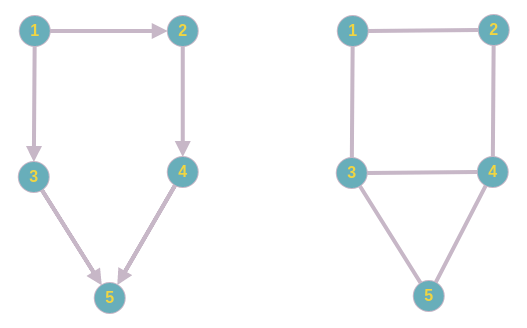
\includegraphics[scale=0.3]{wrs_non_chordal_example.png}
  \caption{An example of a DAG whose moral graph is non-chordal.}
  \label{fg:wrs_non_chordal}
\end{figure}
For any given DAG $G$, it has a unique moral graph $F$ s.t. $B_V^G=B_V^F$. Figure \ref{fg:wrs_non_chordal} is an example of a DAG and its moral graph, which is non-choral. Hence, $\phi$ is non-surjective. \qed
\end{proof}

\section{Weak recursively simplicial graphs}
\begin{definition}
\label{def:collider}
A \textbf{collider} in a hybrid graph is a node with at least two parents. 
\end{definition}

\begin{definition}
\label{def:consistent_ext}
A DAG $G$ is a \textbf{consistent extension} of a hybrid graph $H$ if $G$ and $H$ have the same skeleton and the same set of colliders. 
\end{definition}

Let $F=(V,E)$ be a graph over $n$ nodes. Let $S=\{S_1, \dots, S_m\}$ be a set of disjoint subsets of $V$ s.t. $\cup_{i=1}^m S_i=V$. Let $U=\{U_1, \dots, U_m\}$ be a set of disjoint subsets of $E$, where $U_i \subseteq \{v_jv_k \mid \forall v_j, v_k \in N_l, \forall v_l \in S_i\}$. Two extremes of $U_i$ are the empty set and the edges between all pairs of neighbours of $v_l$ for all $v_l \in S_i$. We use $O = \{(S_1, U_1), \dots, (S_m, U_m)\}$ to denote the pairs. Next we introduce a subset of undirected graphs which are not as strong as recusrively simplicial.  

\begin{definition}
\label{def:wrs}
A graph $F=(V,E)$ is \textbf{weak recursively simplicial (WRS)} if there exits $O = \{(S_1, U_1), \dots, (S_m, U_m)\}$ such that $S_1$ is the set of simplicial nodes in $F$ and $S_{i}$ is the set of simplicial nodes in the subgraph obtained by removing from $F$ the pairs $\{O_1, \dots, O_{i-1}\}$ for $i \in [2,m]$. 
\end{definition}
The reason such a graph is named weak recursively simplicial is because if we only remove the simplicial nodes from $F$, the induced subgraph over the remaining nodes may or may not have any simplicial nodes. So none or some edges between neighbours of simplicial nodes may need to be removed as well to retain the recursion. By definition, a chordal graph is also weak recursively simplicial by letting $U_i=\emptyset$. The converse, however, is not true. The graph on the right of Figure \ref{fg:wrs_non_chordal} is a WRS graph. It has $O_1 = \{S_1=\{5\}, U_1=\{3-4\}\}$. The subgraph obtained by removing $O_1$ is a chordal graph that is also WRS. Therefore, the original graph is WRS.  

\begin{proposition}
\label{prop:moral_implies_wrs}
Let $G=(V,E)$ be a DAG and $F$ be the moral graph of $G$. Then $F$ is weak recursively simplicial. 
\end{proposition}

\begin{proof}
(Base case) $G(1) = F(1)$ is a single node graph, so $F(1)$ is WRS. (Inductive hypothesis) Assuming the moral graph $F(n)$ of any DAG $G(n)$ with $n$ nodes is WRS. (Inductive step) Adding the node $v_{n+1}$ in $G(n)$ as a new leaf produces another DAG $G(n+1)$ with $n+1$ nodes. Since $v_{n+1}$ is a leaf in $G(n+1)$, it becomes a simplicial node in $F(n+1)$ after moralization. In addition, extra edges may be introduced to connect parents of $v_{n+1}$. Since $v_{n+1}$ is a simplicial node, it can be removed from $F(n+1)$ together with the extra edges introduced. Hence, we get back to the same moral graph $F(n)$ that is assumed to be WRS. Therefore, $F(n+1)$ is also WRS. \qed
\end{proof}
Proposition \ref{prop:moral_implies_wrs} suggests that the moral graph of any DAG is WRS. To prove there is a one-to-one correspondance between moral graphs and WRS graphs, we want to show that the converse is also true. That is, a WRS graph $F$ can be oriented into a DAG $G$ (possibly with some edge removal) such that the moral graph of $G$ is identical to $F$. 

\begin{proposition}
\label{prop:wrs_implies_moral}
Let $F=(V,E)$ be a weak recursively simplicial graph. Then $F$ is the moral graph of a DAG. 
\end{proposition}

\begin{proof}
(Base case) $F(1)$ is a single node WRS graph, and also the moral graph of the single node DAG $G(1)$. (Inductive hypothesis) Assuming any WRS graph $F(n)$ with $n$ nodes is the moral graph of a DAG $G(n)$. (Inductive step) Adding $v_{n+1}$ into $F(n)$ as a simplical node, so the resulting graph $F(n+1)$ is WRS. Since $v_{n+1}$ is a simplicial node, there exists a DAG $G(n+1)$, in which $v_{n+1}$ is a leaf. Therefore, the moral graph of $G(n+1)$ is $F(n+1)$. \qed

%$F$ is WRS implies the neighbours of a simplicial node in each  step can be directed towards the simplicial node. The resulting graph after recurtion is a hybrid graph $H$, the undirected edges in which are between neighbours of simplicial node. In addition, the two end nodes of any undirected edges must not be simplicial nodes. For otherwise, the edges would have been directed too. Therefore, $H$ must have a DAG extension $G$ which has the same skeleton and set of colliders as $H$. Since the edges removed are between spouses whose common child is a simplicial node, we have $B_G = B_F$. Therefore, $F$ is the moral graph of $G$. \qed
\end{proof}

\begin{corollary}
\label{cor:wrs_equal_moral}
An undirected graph is weak recursively simplicial if and only if it is the moral graph of a DAG. 
\end{corollary}
\begin{proof}
The corollary follows from the Proposition \ref{prop:moral_implies_wrs} and Proposition \ref{prop:wrs_implies_moral}. \qed
\end{proof}

\begin{corollary}
Let $\mathcal{F}=\{F=(V,E) \mid F \text{ is weak recursively simplicial}\}$ be the set of weak recursively simplicial graphs over $V$ and $\mathcal{B} = \{B_V^G \mid \text{for all DAG $G$ over $V$}\}$ be the set of Markov blanket families of any DAG over $V$. Then $|\mathcal{F}| = |\mathcal{B}|$. 
\end{corollary}
\begin{proof}
It is straightforward that there is a one-to-one correspondance between $\mathcal{B}$ and moral graphs. Hence, Corollary \ref{cor:wrs_equal_moral} implies that $\mathcal{F}$ has a one-to-one correspondance with $\mathcal{B}$, so equal cardinality. \qed
\end{proof}

Next, we present a backtracking algorithm for checking whether or not a given graph $F=(V,E)$ is WRS. If it is, the algorithm will find a DAG $G$, the moral graph of whom is $F$. Notice that this algorithm may produce a hybrid graph, which always has a consistent DAG extension according to Proposition \ref{prop:wrs_implies_moral}. Hence, we use the algorithm presented in \cite{dor1992simple} to get it. 
\begin{algorithm}[]
\caption{Backtracking algorithm to test WRS of graphs}
\label{alg:wrs_bktr}
\begin{algorithmic}[]
	\Require{$F$ is an undirected graph obtained by connecting all $v_j \in B_i$ with $v_j, \forall v_j \in V$}
    \Statex
    \Function{$WRS$}{$F$}
    \If{$F$ is chordal} 
    	\Return {TRUE} 
    \EndIf
    \State Find all the set $S$ of all simplicial nodes in $F$
    \If{$S \neq \emptyset$} 
    	\State Find $E=\{v_jv_k \mid \forall v_j, v_k \in N_i, \forall v_i \in S\}$
    	\State $backup = F$
    	\ForEach{$U \subseteq E$} \Comment{for each subset of $E$}
    	\State $F=backup$
    	\State $F=F-S-U$ \Comment{Remove simplicial nodes $S$ and edges $U$}
        \If{$WRS(F)=$ TRUE}
        	\Return {TRUE}
        \EndIf
      \EndFor
    \EndIf
    \State \Return{FALSE}
    \EndFunction
\end{algorithmic}
\end{algorithm}

\cite{verma1992algorithm} did similar work but for finding consistent DAG with the set of conditional independencies. It maybe equivalent to MBs?



\iffalse
\section{Unique prime decomposition}
The concept of simplicial decomposition of graphs was discussed by \cite{wagner1937eigenschaft}, \cite{halin1964simpliziale}, and \cite{diestel1987simplicial}. One of the important proofs is that any finite graphs (don't care about infinite graphs) has a prime decomposition, and such prime decomposition is unique. 
\fi

\section{Some random notes}

\textbf{Lloyd's conjecture:} knowing a graph is wrs, adding an edge to obtain a supergraph, perhaps it is efficient to check if the supergraph is wrs.

\begin{proof}
because remove the added edge, then we obtain the original graph which we know is wrs. however, we don't remove a random edge when checking wrs unless the edge connects to a simplicial node. what if the edge is not connected with a sim node? if we know the original graph is wrs and we know the set of sim nodes in the recursion and the set of edges to delete, then we could easily check if the new edge is connected with any one of the sim node, if it is then good. if not, then we could check if the new edge is connected with two neighbours of a sim node, if it is then good. if a graph is wrs, then it eventually will diminish, so the new edge must appear somewhere in the recursion to either stop the recursion or don't stop it.
\end{proof} 

\begin{corollary}
DAGs in the same Markov equivalent class produce the same Markov blanket sets $B_X$. 
\end{corollary}
\begin{proof}
If two DAGs $G_1$ and $G_2$ are Markov equivalent, they have the same skeleton and the same set of colliders. This implies $B_i^{G_1} = B_i^{G_2}, \forall X_i \in X$. \qed
\end{proof}
Notice that two Markov equivalent classes could entail the same $B_X$. For example... 

\begin{corollary}
$|\{\text{chordal graphs}\}| \le |B_X| \le |\{\text{Markov equivalent classes}\}|$.
\end{corollary} 

Counting labelled chordal graphs \cite{wormald1985counting}, counting Markov equivalent classes (assymptotic ratio of around 0.27 to DAGs) \cite{gillispie2001enumerating}. 

\begin{table}[]
\centering
\caption{Comparison between the number of chordal graphs , the number of weak recursively simplicial graphs, the number of undirected graphs and the number of Markov equivalent classes.}
\label{my-label}
\begin{tabular}{lllll}
\# nodes & \# chordal graphs & \# weak r.s. graphs & \# undirected graphs & \# Markov equivalent classes \\ \hline
1        & 1                 & 1          & 1         & 1 \\
2        & 2                 & 2          & 2         & 2 \\
3        & 8                 & 8          & 8         & 11 \\
4        & 61                & 61         & 64         & 185 \\
5        & 822               & 882        & 1024            & 8782\\
6        & 18154             &       & 32768              & 1067825\\
7        & 617675            &            & 2097152         & 312510571\\
8        & 30888596          &            &  268435456        & 212133402500 \\
9        & 2192816760        &            &  68719476736       & 326266056291213 \\ 
10       & 215488096587 ($2\times 10^{11}$)     &            &  35184372088832 ($3\times 10^{13}$)       & 118902054495975141 ($1\times 10^{17}$) \\ \hline
\end{tabular}
\end{table}

\begin{proposition}
\label{prop:leaf_is_sim}
Let $G$ be a DAG and $F$ be the moral graph of $G$. If a node $x$ is a leaf in $G$, then it must be a simplicial node in $F$. 
\end{proposition}
\begin{proof}
If $x$ is a leaf in $G$, it has only parents, which form a clique after moralization. By definition, $x$ is a simplicial node in $F$. \qed
\end{proof}

\begin{corollary}
Let $G$ be a DAG and $F$ be the moral graph of $G$. Then $F$ must have at least one simplicial node. 
\end{corollary}

\begin{proof}
Since each DAG has at least one leaf, by Proposition \ref{prop:leaf_is_sim} $F$ have at least one simplicial node. \qed
\end{proof}

\begin{corollary}
\label{cor:negation_of_leaf_is_sim}
Let $G$ be a DAG and $F$ be the moral graph of $G$. If a node $x$ is not a simplicial node in $F$, then it must not be a leaf in $G$. 
\end{corollary}

\begin{proposition}
Let $G$ be a DAG and $F$ be the moral graph of $G$. Let $S^1$ be the set of simplicial nodes in $F$ and $F_1$ be the induced subgraph of $F$ over $X\setminus S^1$. Then there must exist at least one simplicial node after removing from $F'$ all the edges between $N(X_i), \forall X_i \in S^1$.
\end{proposition}

\begin{proof}
Let $F_1'$ be the result of removing from $F_1$ all the edges between $N(X_i), \forall X_i \in S^1$. The corresponding directed graph $G'$ of $F_1'$ must be a subgraph of the DAG $G$, so also acyclic. Assuming $F_1'$ has no simplicial nodes, by Corollary \ref{cor:negation_of_leaf_is_sim} $G'$ has no leaf, which is a contradiction. \qed
\end{proof}


Here are some issues worth discussing:
\begin{enumerate}
\item Application: the backtracking algorithm can now be applied when learning MBs in paralle. What if there are conflicts between two MBs, which one should give up? Need to estimate uncertainty?
\item Simplicial nodes in the first step always contain the leaves.
\item Those nodes that become simplicial in the next step without having to delete any edges contain the leaves in the next step. 
\item So wrs can be used to test if a MB family is consistent with a DAG, it would be good if we can also find out how many consistent DAGs or essential graphs are there for this MB family. 
\item also it would be good if we can explore wrs into details, such as what dag nodes become simplicial nodes in wrs recursion, and if no edges need to be deleted from a simplicial node's neighbours then what's this simplicial node?
\item maybe there is a path from s.t. every step is a moral graph of a dag, perhaps can be proved by delete an edge from a dag.   
\end{enumerate}

\textbf{Questions:} If a graph $F$ is known to be wrs, does is help to decide if a subgraph/supergraph different by one edge from $F$ is wrs or not?

\textbf{Answer:} Probably not. If it is, then we know a base case, any graph can be reached from this base case, hence any graph can be efficiently tested. 

\iffalse
The undirected edge connects two parents of a common child is called a \textit{moralized edge}. The process of obtaining a moral graph from a DAG is called \textit{moralization}. There is a unique moral graph of each DAG. Next, we define the reverse of a moralization process as \textit{demoralization}. It is defined on undirected graphs with at least one simplicial node. 
\fi

\section{Notations}
\subsection{Notations}
\begin{table}[]
\centering
\caption{Notations}
\label{my-label}
\begin{tabular}{ll}
\hline
$F$ &  a undirected graph \\
$G$ & a DAG \\
$X$ & a set of random variables (nodes) \\
$X_i$ & a random variable (or node) in $X$ \\
$X_{-i}$ & $X \setminus X_i$ \\ 
$X_{-[1,\dots, i]}$ & $X \setminus \{X_1, \dots, X_i\}$ \\ 
$B_i^G$ & the Markov blanket of a variable $X_i$ in $G$ \\ 
$B_X^G$ & $\{B_i \mid \forall X_i \in X\}$ \\ \hline
\end{tabular}
\end{table}

\bibliographystyle{named}
\bibliography{/home/kl/Documents/causal_discovery_ref_list}

\end{document}